\documentclass[final]{beamer}
\usepackage[scale=1.24]{beamerposter}
\usetheme{confposter}
\setbeamercolor{block title}{fg=purple,bg=white}
\setbeamercolor{block body}{fg=black,bg=white}
\setbeamercolor{block alerted title}{fg=white,bg=purple!70}
\setbeamercolor{block alerted body}{fg=black,bg=purple!10}

\newlength{\sepwid}
\newlength{\onecolwid}
\newlength{\twocolwid}
\newlength{\threecolwid}
\setlength{\paperwidth}{36in} % A0 width: 46.8in
\setlength{\paperheight}{48in} % A0 height: 33.1in
\setlength{\sepwid}{0.024\paperwidth} % Separation width (white space) between columns
\setlength{\onecolwid}{0.22\paperwidth} % Width of one column
\setlength{\twocolwid}{0.464\paperwidth} % Width of two columns
\setlength{\threecolwid}{0.708\paperwidth} % Width of three columns
\setlength{\topmargin}{-0.5in} % Reduce the top margin size
%-----------------------------------------------------------

\usepackage{graphicx}  % Required for including images

\usepackage{booktabs} % Top and bottom rules for tables

%----------------------------------------------------------------------------------------
%	TITLE SECTION 
%----------------------------------------------------------------------------------------
\title{Where's Waldo?: A Machine Learning Approach to a Classic Childhood Problem} % Poster title

\author{Thomas Rhines} % Author(s)

\institute{https://github.com/tjrhines/Final\_Public} % Institution(s)

\logo{\pgfputat{\pgfxy(-74,107)}{\pgfbox[center,base]{\includegraphics[width=7cm]{pictures/waldo.png}}}}  


%----------------------------------------------------------------------------------------

\begin{document}

\addtobeamertemplate{block end}{}{\vspace*{2ex}} % White space under blocks
\addtobeamertemplate{block alerted end}{}{\vspace*{2ex}} % White space under highlighted (alert) blocks

\setlength{\belowcaptionskip}{2ex} % White space under figures
\setlength\belowdisplayshortskip{2ex} % White space under equations

\begin{frame}[t] % The whole poster is enclosed in one beamer frame

\begin{columns}[t] % The whole poster consists of three major columns, the second of which is split into two columns twice - the [t] option aligns each column's content to the top

\begin{column}{\sepwid}\end{column} % Empty spacer column

\begin{column}{\onecolwid} % The first column

%----------------------------------------------------------------------------------------
%	Intro
%----------------------------------------------------------------------------------------
\begin{alertblock}{Introduction}

Waldo is hard to find. Why not let a computer do it? In this project, I demonstrate that a U-Net neural network can segment and localize Waldo in complex images. Overall, a neural network and simple localization algorithm is able to find Waldo.

\end{alertblock}

\begin{block}{Network}

\begin{figure}
    %\centering
    \includegraphics[width=1.05\textwidth]{pictures/unet.png}
    \caption{U-Net architecture used for segmentation (http://lmb.informatik.uni-freiburg.de/Publications/2015/RFB15a/)}
    \label{fig:unet}
\end{figure}

The network used was based on the U-Net architecture in Ronneberger et al.'s paper \cite{DBLP:journals/corr/RonnebergerFB15}. This network was developed for medical image segmentation, and \textbf{performs well on small datasets}. Much of the network architecture code was obtained and modified from Sterbak's website \cite{manual}. The network consists of a contracting path, which repeats a block of a convolutional layer, followed by a ReLU layer and downsampled with a max pooling layer. \textbf{The contracting path is sensitive to image context}. An expansive path uses up-convolutional layers, followed by a concatenation with the symmetric layer and another convolutional and ReLU layer. \textbf{The expansive path enables precise localization}, making this network ideal for small dataset image segmentation. Batch normalization was added after each layer.
\end{block}





\begin{figure}
    \centering
    \includegraphics[width=\textwidth]{pictures/loss.png}
    \caption{Training and validation loss metrics}
    \label{fig:loss}
\end{figure}



\end{column}


\begin{column}{\sepwid}\end{column} % Empty spacer column

\begin{column}{\onecolwid}

%----------------------------------------------------------------------------------------
%	Network
%----------------------------------------------------------------------------------------




%----------------------------------------------------------------------------------------
%	Data
%----------------------------------------------------------------------------------------
\begin{block}{Data}



The data for this project came from six "Where's Waldo?" books [\textbf{2}]. The books were scanned at 5100 x 3300 pixels. Of the six books, five were included in the dataset and one exclusively for testing. Truth masks for all training images were made using Matlab. An example is shown in Figure \ref{fig:datagen}. The training dataset was split randomly into 65\%  training, 20\% validation, and 15\% testing. A data generator was created to randomly flip the training images horizontally, and take a random 256x256 pixel crop that contains Waldo. In addition to preserving image resolution, this step ensures that Waldo's location in the training images is different each time the network sees it, avoiding training location biases. Horizontal flipping effectively doubles the dataset. 

\vspace{0.6in}

\begin{figure}
    \centering
    \includegraphics[width=0.8\textwidth]{pictures/datagen.png}
    \caption{Example data generator output used for training network. Both horizontal flipping and cropping are used.}
    \label{fig:datagen}
\end{figure}




\end{block}



\begin{block}{Methods}

The network was implemented in Python using the Keras library. The network was trained with a batch size of 16 images for 30 epochs of 20 steps each. Training took about two hours on a CPU. An "Adam" optimizer was used. Loss metrics were calculated as the binary cross-entropy for pixel outputs. The training loss history is shown in Figure \ref{fig:loss}.







\end{block}

\end{column}



\begin{column}{\sepwid}\end{column} % Empty spacer column

\begin{column}{\twocolwid} % Begin a column which is two columns wide (column 2)



%----------------------------------------------------------------------------------------
%	Results
%----------------------------------------------------------------------------------------

\begin{block}{Evaluation}

Three separate methods were used to evaluate performance of the model: 
\begin{itemize}
    \item Testing on images originally allocated in training data, cropping them randomly around Waldo. Results can be seen in Figure \ref{fig:results}. Using the predicted and truth masks, I calculated the intersection over union (IOU) for all images. The \textbf{mean IOU is 0.748} for these seven images, suggesting reasonably good results with a very small dataset and few training epochs. 
    
    \item I developed a simple algorithm to tile the input of a larger image and input each tile into the network. The largest area object in the prediction was classified as Waldo. This algorithm found Waldo in all seven original testing images.
    
    \item The same algorithm was used for the independent, untrained Waldo book. Waldo was found 3/6 times, Wenda was found 2/6 times (a near-success) and Waldo was not found 1/6 times. Examples are shown in Figure \ref{fig:examples}.
\end{itemize}

\end{block}



\begin{alertblock}{Results}
\begin{columns}[t,totalwidth=0.95\twocolwid] % Split up the two columns wide column
\begin{column}{0.6\onecolwid}\vspace{-.6in}
\begin{figure}
    \centering
    \includegraphics[width = 1.1\textwidth]{pictures/results.png}
    \caption{Input images, truth masks, and predictions for  original testing set}
    \label{fig:results}
\end{figure}
\end{column}

\begin{column}{1.3\onecolwid}\vspace{0in}

\begin{figure}
    \centering
        
        \begin{subfigure}{\textwidth}
        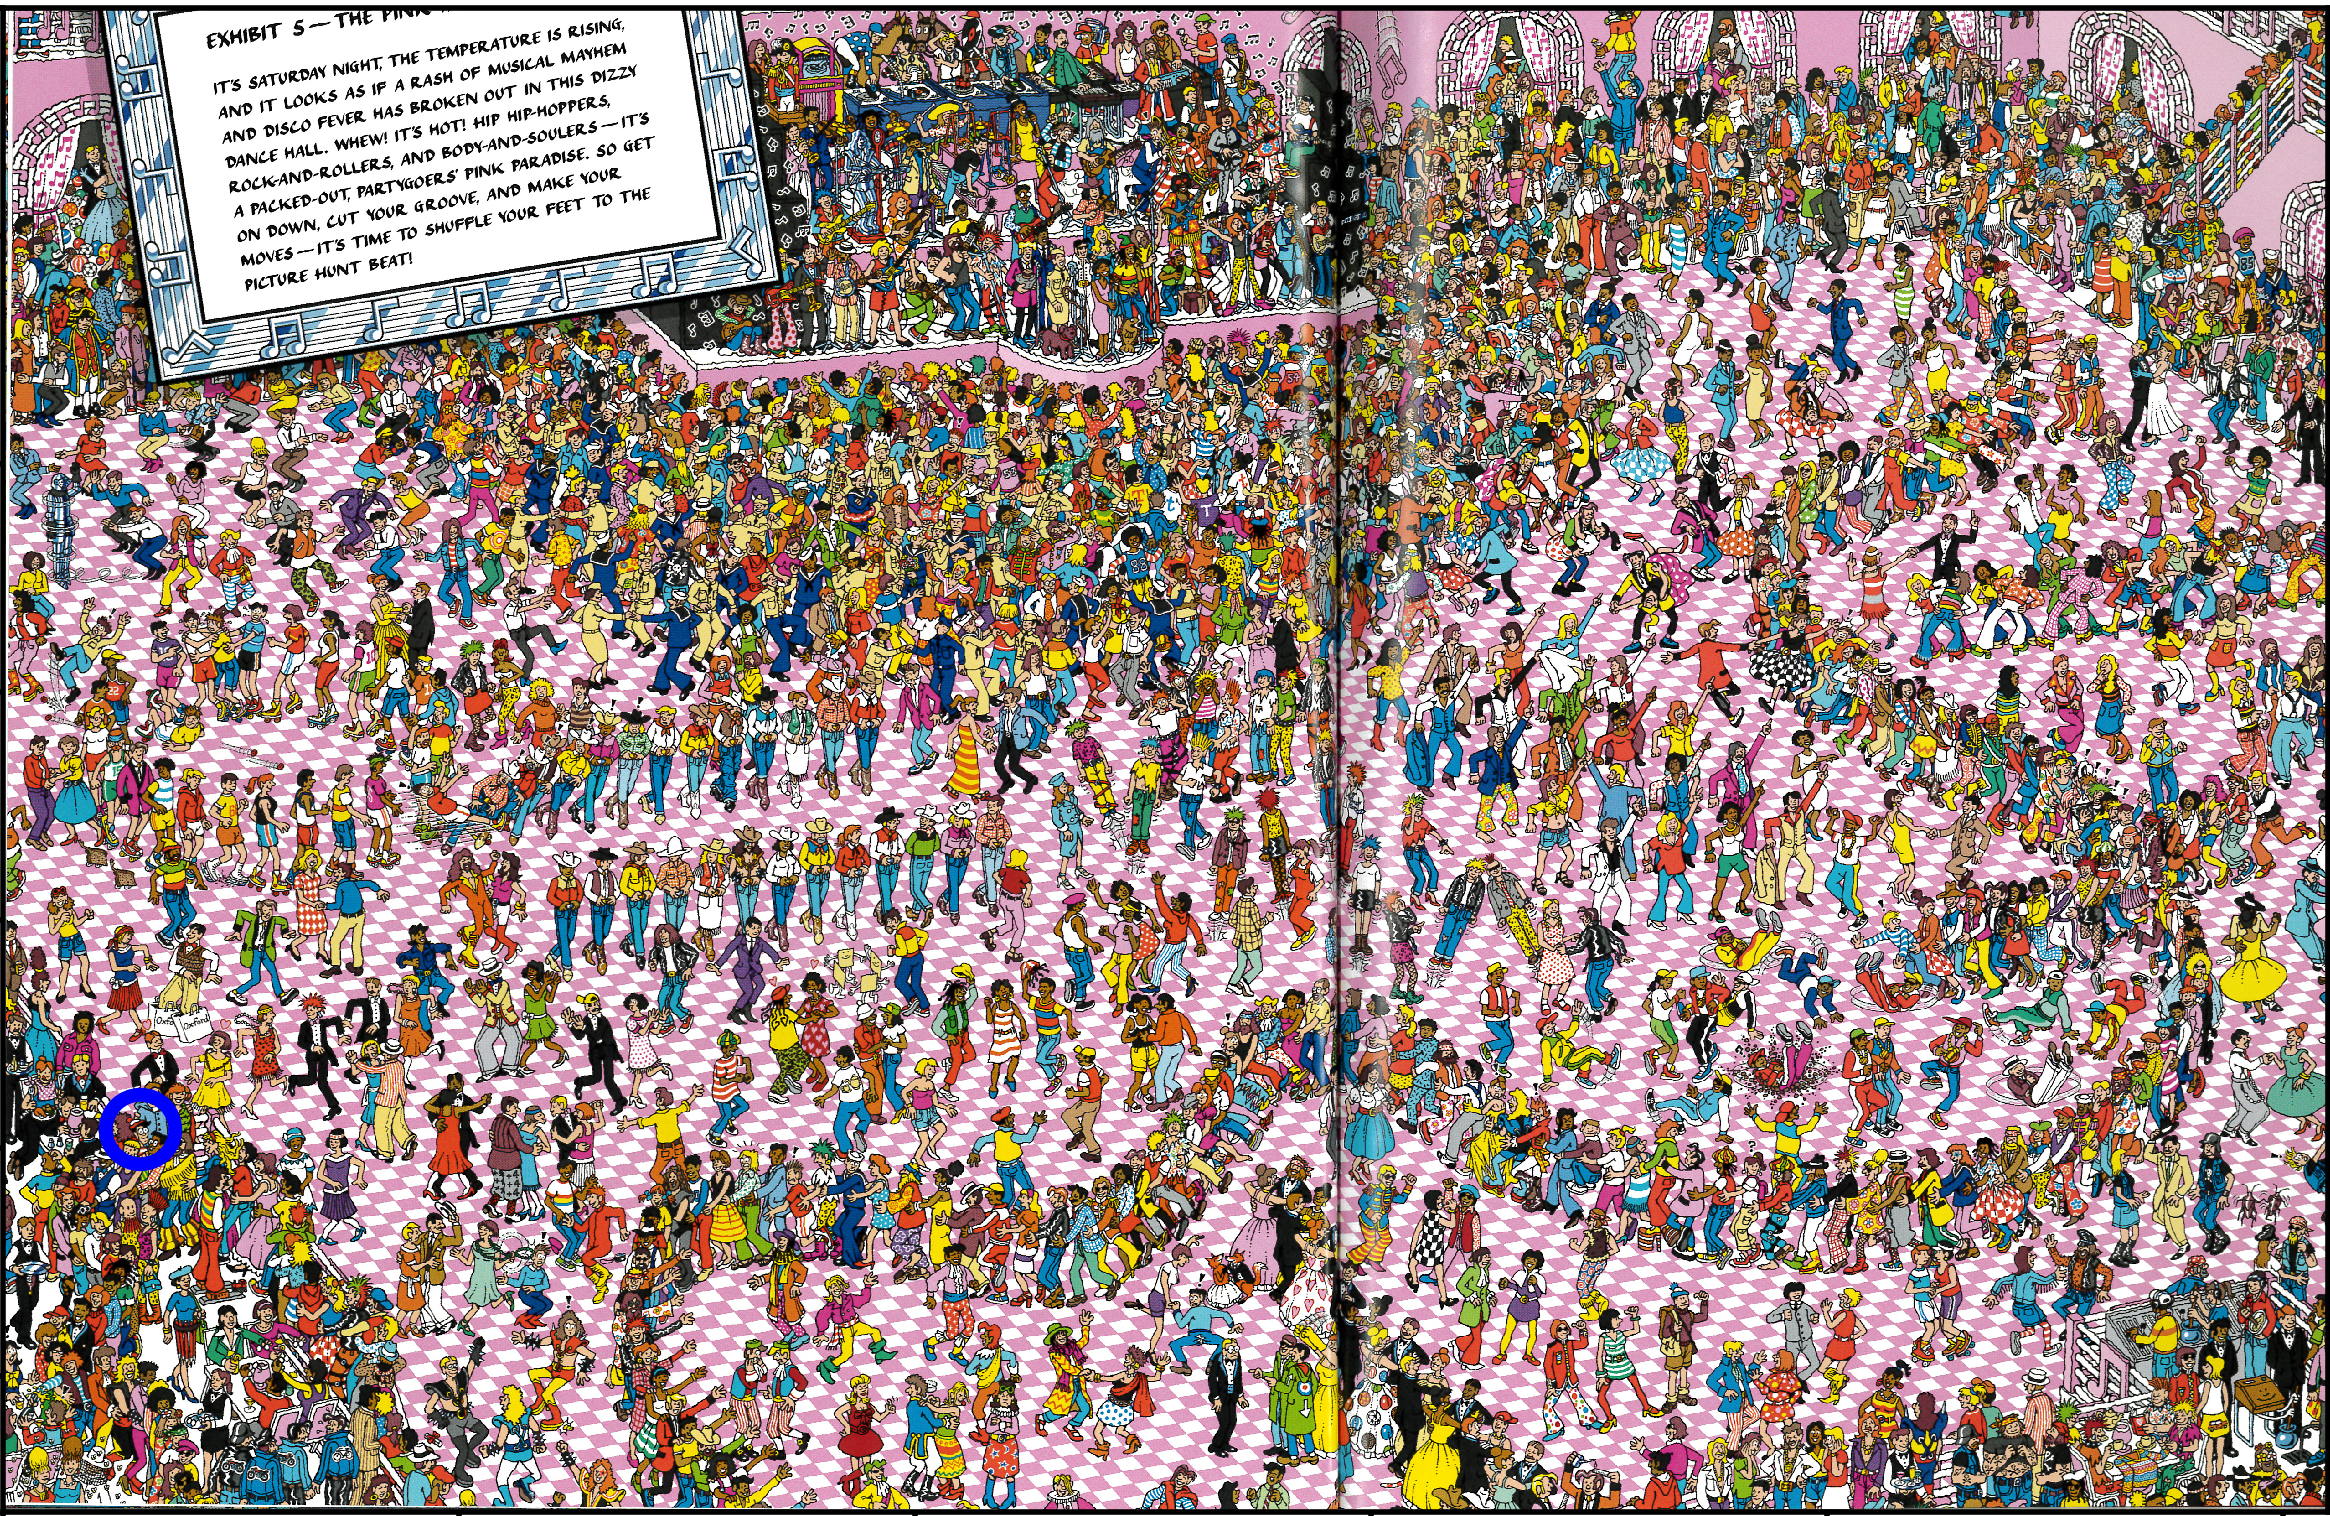
\includegraphics[width=\textwidth]{pictures/example3.png} \\
        \end{subfigure}
        
        \begin{subfigure}{\textwidth}
        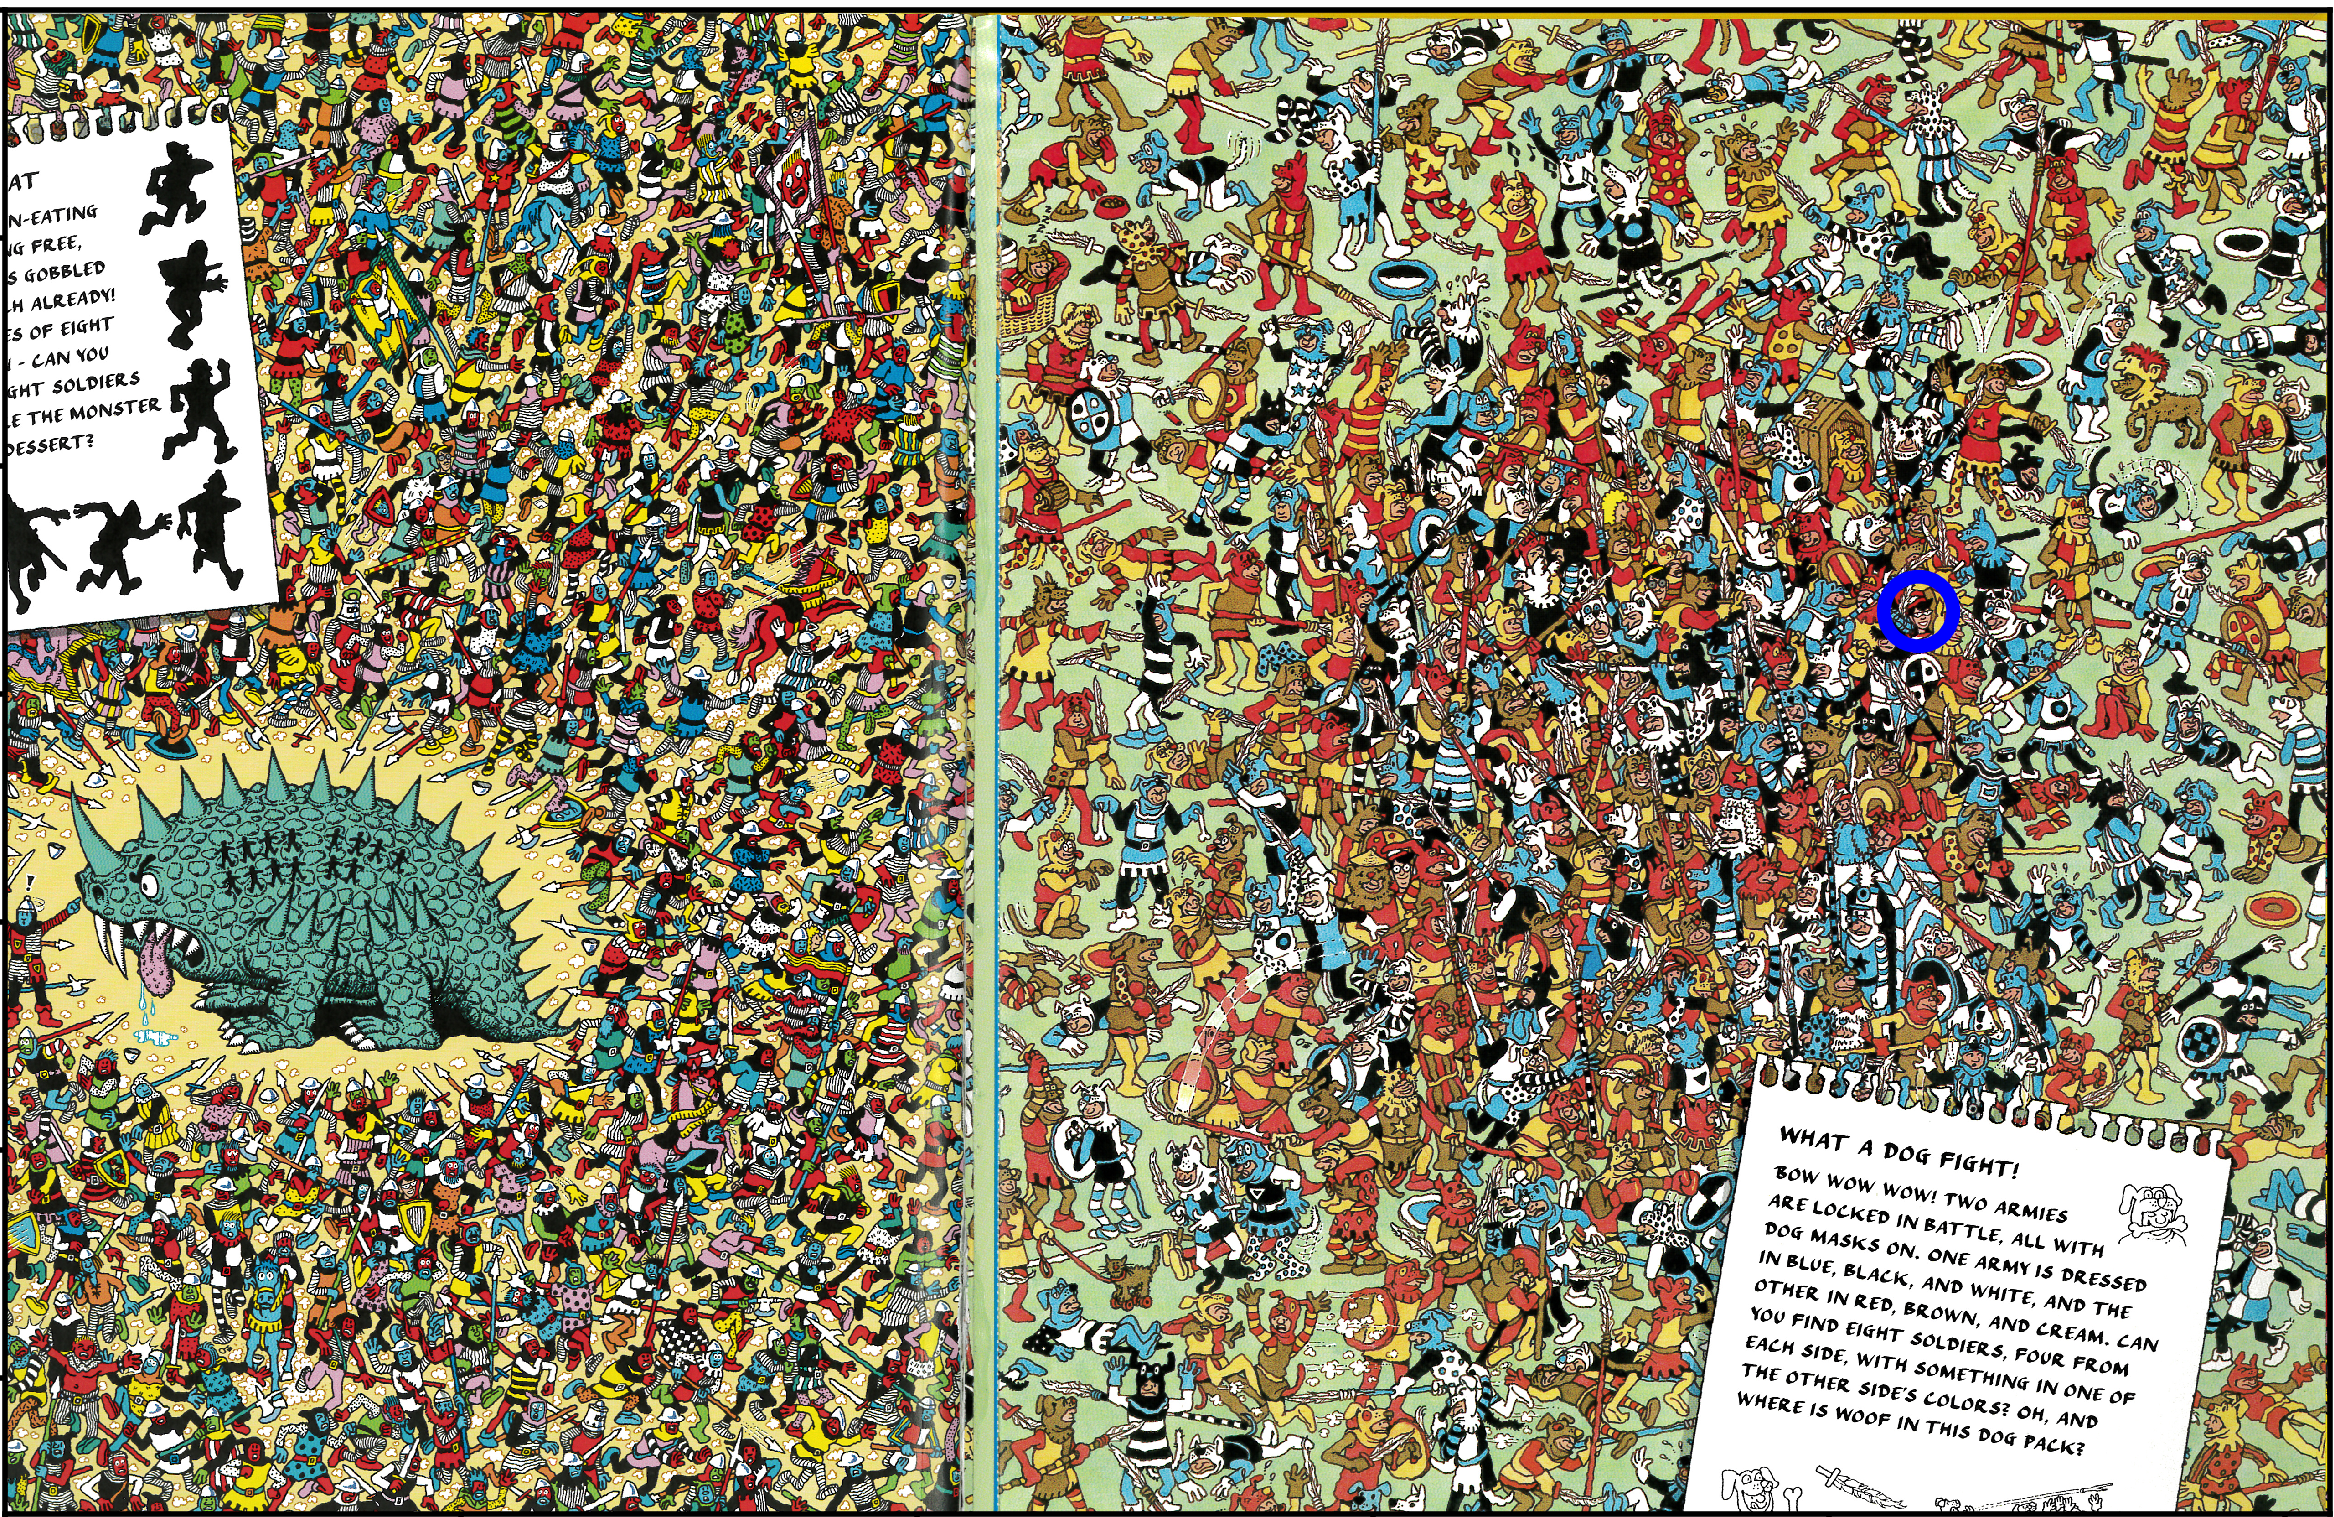
\includegraphics[width=\textwidth]{pictures/example10.png}
        \end{subfigure}

        
        
    \caption{Example results of the tiling algorithm. The first is a correct localization from the original test set. The second image, from the independent testing book, finds Wenda.}
    \label{fig:examples}
\end{figure}



\end{column}
\end{columns}
\end{alertblock}


\begin{columns}[t,totalwidth=\twocolwid] % Split up the two columns wide column
\begin{column}{\onecolwid}\vspace{-.6in}


\begin{block}{Conclusion}

This project shows that neural networks are able to identify and localize objects in complicated visual data. Results are primarily qualitative, and successfully identify the target in most tests. Waldo is a 'toy model" for bigger problems, which are relevant to physics. Medical physicists segment diseases in medical images, and astrophysicists automatically probe huge quantities of stellar images. Applications of neural networks are applicable whenever image data is available.

\end{block}




\end{column}

\begin{column}{\onecolwid}\vspace{-.6in}



\begin{block}{References}

\nocite{*} % Insert publications even if they are not cited in the poster
\small{\bibliographystyle{unsrt}
\bibliography{sample}\vspace{0.75in}}


\end{block}

\vspace{-1in}
\begin{block}{Acknowledgements}
Special thanks to my dad for scanning the "dataset"
\end{block}
\end{column}

\end{columns}



\end{column}





\end{columns}
\end{frame}




\end{document}